\section{Approfondissement du mod\`ele}

\subsection{Limites du mod\`ele de base et objectif du raffinement}
Le mod\`ele de base d\'ecrit en Section~III repose sur une seule couche convolutionnelle suivie d'un \textit{flattening} et d'une t\^ete dense. Cette structure reste valide pour une premi\`ere \'etude, mais elle pr\'esente trois limites nettes pour la classification sur CIFAR-10. D'abord, l'extraction de caract\'eristiques demeure peu hi\'erarchique, puisqu'une seule convolution est appliqu\'ee avant la d\'ecision. Ensuite, l'essentiel des param\`etres entra\^inables est concentr\'e dans la partie dense : sur $132010$ param\`etres, $131786$ appartiennent \`a la t\^ete dense, contre seulement $224$ pour la couche convolutionnelle. Enfin, aucune r\'egularisation effective n'intervient dans cette baseline, puisque les taux de \textit{dropout} et les coefficients $L^2$ sont nuls.

Les architectures convolutionnelles sont pourtant motiv\'ees, dans le cadre du cours, par l'id\'ee d'une extraction locale et invariante par translation au moyen d'un banc de filtres, combin\'ee \`a des m\'ecanismes de r\'eduction spatiale par \textit{pooling} ou \textit{stride} \cite{manzanera_classification_apprentissage,poly_chap4_classifml,lecun_convolutional_networks}. L'approfondissement du r\'eseau doit donc permettre \`a la fois d\'augmenter le champ r\'ecepteur effectif, de construire des repr\'esentations plus abstraites et de r\'e\'equilibrer la r\'epartition des param\`etres entre la partie convolutionnelle et la partie d\'ecisionnelle. L'objectif de cette section consiste ainsi \`a concevoir une architecture plus profonde, \`a en v\'erifier la coh\'erence dimensionnelle, puis \`a mesurer rigoureusement si le gain de performance justifie la complexit\'e suppl\'ementaire.

\subsection{Conception d'une architecture convolutionnelle plus profonde}
Le raffinement a \'et\'e men\'e \`a partir de trois variantes plus profondes que la baseline. La premi\`ere, not\'ee $M1$, ajoute une deuxi\`eme \'etape convolutionnelle et porte la profondeur \`a quatre convolutions. La deuxi\`eme, not\'ee $M2$, ajoute une troisi\`eme \'etape convolutionnelle, ce qui porte la profondeur \`a six convolutions et r\'eduit la r\'esolution finale \`a $4\times 4$. La troisi\`eme, not\'ee $M3$, reprend exactement le squelette de $M2$ mais y ajoute une r\'egularisation explicite : \textit{dropout} de $0.25$ apr\`es chaque \textit{pooling}, \textit{dropout} de $0.5$ avant la couche dense cach\'ee et p\'enalisation $L^2$ de coefficient $10^{-4}$.

Cette progression respecte l'interpr\'etation du cours : les couches convolutionnelles successives apprennent des \textit{features} de complexit\'e croissante, tandis que les couches de \textit{pooling} r\'eduisent la r\'esolution spatiale et augmentent la port\'ee contextuelle des neurones profonds \cite{poly_chap4_classifml}. Le choix de noyaux $3\times 3$ conserv\'es \`a toutes les couches maintient un calcul local simple, tandis que la multiplication des \'etapes convolutionnelles permet d\'agrandir progressivement le champ r\'ecepteur sans introduire de filtres tr\`es larges. Le tableau~\ref{tab:section6_architectures} r\'esume les variantes compar\'ees.

\begin{table*}[htbp]
\centering
\caption{Architectures compar\'ees pour l'approfondissement du mod\`ele.}
\label{tab:section6_architectures}
\small
\begin{tabular}{|c|l|l|c|}
\hline
Mod\`ele & Backbone convolutionnel & R\'egularisation & Param\`etres \\
\hline
$M0$ & $8$/pool & aucune & $132010$ \\
$M1$ & $16$-$16$/pool $\rightarrow$ $32$-$32$/pool & aucune & $148442$ \\
$M2$ & $16$-$16$/pool $\rightarrow$ $32$-$32$/pool $\rightarrow$ $64$-$64$/pool & aucune & $138330$ \\
$M3$ & $16$-$16$/pool $\rightarrow$ $32$-$32$/pool $\rightarrow$ $64$-$64$/pool & dropout $0.25/0.25/0.25$, dropout dense $0.5$, $L^2=10^{-4}$ & $138330$ \\
\hline
\end{tabular}
\end{table*}

Deux observations ressortent imm\'ediatement. D'une part, $M1$ poss\`ede davantage de param\`etres que $M3$, bien qu'il soit moins profond ; cela provient du fait que deux seuls \textit{poolings} laissent une carte finale de taille $8\times 8\times 32$, soit un \textit{flattening} de dimension $2048$, alors que $M3$ descend \`a $4\times 4\times 64$, soit une dimension $1024$ avant la partie dense. D'autre part, $M2$ et $M3$ ont exactement le m\^eme nombre de param\`etres, puisque \textit{dropout} et p\'enalisation $L^2$ n'ajoutent pas de poids entra\^inables.

\subsection{Coh\'erence dimensionnelle des tenseurs}
La coh\'erence entre les tenseurs d'entr\'ee et de sortie a \'et\'e contr\^ol\'ee explicitement pour toutes les architectures. Si une couche re\c coit un tenseur $H_l \times W_l \times C_l$, alors une convolution $3\times 3$ avec \texttt{padding="same"} et pas $1$ produit un tenseur $H_l \times W_l \times F_l$, o\`u $F_l$ d\'esigne le nombre de filtres. Un \textit{max pooling} $2\times 2$ de pas $2$ produit ensuite un tenseur
\begin{equation}
\frac{H_l}{2} \times \frac{W_l}{2} \times C_l,
\end{equation}
ce qui impose que les dimensions spatiales restent compatibles avec les r\'eductions successives.

Pour le mod\`ele finalement retenu, la cha\^ine dimensionnelle s'\'ecrit :
\begin{equation}
\resizebox{0.98\columnwidth}{!}{$
\begin{aligned}
32\times 32\times 3 &\rightarrow 32\times 32\times 16 \rightarrow 32\times 32\times 16 \rightarrow 16\times 16\times 16, \\
16\times 16\times 16 &\rightarrow 16\times 16\times 32 \rightarrow 16\times 16\times 32 \rightarrow 8\times 8\times 32, \\
8\times 8\times 32 &\rightarrow 8\times 8\times 64 \rightarrow 8\times 8\times 64 \rightarrow 4\times 4\times 64, \\
4\times 4\times 64 &\rightarrow 1024 \rightarrow 64 \rightarrow 10.
\end{aligned}$}
\end{equation}
Le tableau~\ref{tab:section6_dimensions} reprend cette progression couche par couche. La transition vers la partie dense demeure assur\'ee par un \textit{flattening}, conform\'ement au sch\'ema d\'ecrit dans le polycopi\'e pour les t\^aches de classification \`a sortie de taille fixe \cite{poly_chap4_classifml}.

\begin{table}[htbp]
\centering
\caption{Coh\'erence dimensionnelle du mod\`ele retenu $M3$.}
\label{tab:section6_dimensions}
\small
\begin{tabular}{|l|c|c|}
\hline
Couche & Sortie & Param\`etres \\
\hline
Input & $32\times 32\times 3$ & $0$ \\
Conv2D $(16)$ & $32\times 32\times 16$ & $448$ \\
Conv2D $(16)$ & $32\times 32\times 16$ & $2320$ \\
MaxPool2D & $16\times 16\times 16$ & $0$ \\
Conv2D $(32)$ & $16\times 16\times 32$ & $4640$ \\
Conv2D $(32)$ & $16\times 16\times 32$ & $9248$ \\
MaxPool2D & $8\times 8\times 32$ & $0$ \\
Conv2D $(64)$ & $8\times 8\times 64$ & $18496$ \\
Conv2D $(64)$ & $8\times 8\times 64$ & $36928$ \\
MaxPool2D & $4\times 4\times 64$ & $0$ \\
Flatten & $1024$ & $0$ \\
Dense & $64$ & $65600$ \\
Dense & $10$ & $650$ \\
\hline
\end{tabular}
\end{table}

\subsection{Protocole d'entra\^inement et comparaison contr\^ol\'ee}
La comparaison a conserv\'e exactement le protocole de donn\'ees de la Section~IV : m\^eme partition r\'eduite de CIFAR-10 ($5000$ images d'entra\^inement, $1000$ de validation, $1000$ de test), m\^eme standardisation image par image et m\^eme nombre de classes. Afin d'isoler autant que possible l'effet de l'architecture, l'optimiseur a \'et\'e fix\'e \`a Adam avec $(\epsilon,\beta_1,\beta_2,\eta)=(10^{-3},0.9,0.999,10^{-7})$, le \textit{batch size} \`a $32$ et le m\'elange des mini-batches \`a \texttt{True}.

La campagne a \'et\'e men\'ee en deux \'etapes. Un \textit{screening} initial a compar\'e les quatre architectures sur la graine $42$ pendant $10$ epochs. Les deux meilleures architectures raffin\'ees ont ensuite \'et\'e soumises \`a une phase de confirmation, avec les graines $42$ et $314$ et un budget de $12$ epochs. La r\`egle de s\'election a \'et\'e fix\'ee \textit{a priori} : accuracy finale de validation moyenne maximale, puis minimum moyen de \textit{val. loss}, puis temps moyen par epoch.

Le tableau~\ref{tab:section6_performance} rassemble les r\'esultats. Lors du \textit{screening}, $M3$ obtient la meilleure accuracy finale de validation ($48.10\%$), devant $M1$ ($46.20\%$), $M2$ ($43.60\%$) et la baseline $M0$ ($39.50\%$). L'int\'er\^et de la r\'egularisation appara\^it d\'ej\`a clairement : $M3$ surpasse $M2$ de $4.5$ points d\'accuracy finale, alors que les deux mod\`eles partagent exactement le m\^eme backbone convolutionnel.

La phase de confirmation confirme cette hi\'erarchie. $M3$ atteint une accuracy finale de validation moyenne de $50.80\% \pm 1.60$, avec un minimum moyen de \textit{val. loss} de $1.4073 \pm 0.0663$. $M1$ progresse lui aussi par rapport \`a la baseline, avec $48.55\% \pm 1.55$, mais reste en retrait. Le gain de $M3$ par rapport \`a $M0$ est de $8.5$ points d\'accuracy finale de validation, au prix d'un temps moyen par epoch qui passe de $1.256\,\mathrm{s}$ \`a $3.708\,\mathrm{s}$.

\begin{table*}[htbp]
\centering
\caption{Comparaison des architectures pendant le \textit{screening} et la confirmation. Pour la confirmation, le symbole $\pm$ d\'esigne l'\'ecart-type empirique sur les deux graines.}
\label{tab:section6_performance}
\small
\begin{tabular}{|c|c|c|c|c|c|c|}
\hline
Etape & Mod\`ele & Nb. conv & Param\`etres & Accuracy finale val. (\%) & Min. val. loss & Temps/epoch (s) \\
\hline
Screening & $M0$ & $1$ & $132010$ & $39.50$ & $1.6113$ & $1.346$ \\
Screening & $M1$ & $4$ & $148442$ & $46.20$ & $1.6386$ & $2.824$ \\
Screening & $M2$ & $6$ & $138330$ & $43.60$ & $1.6178$ & $3.463$ \\
Screening & $M3$ & $6$ & $138330$ & $48.10$ & $1.5431$ & $3.833$ \\
\hline
Confirmation & $M0$ & $1$ & $132010$ & $42.30 \pm 1.10$ & $1.6167 \pm 0.0055$ & $1.256 \pm 0.611$ \\
Confirmation & $M1$ & $4$ & $148442$ & $48.55 \pm 1.55$ & $1.5804 \pm 0.0582$ & $2.478 \pm 0.702$ \\
Confirmation & $M3$ & $6$ & $138330$ & $50.80 \pm 1.60$ & $1.4073 \pm 0.0663$ & $3.708 \pm 1.453$ \\
\hline
\end{tabular}
\end{table*}

\subsection{Mod\`ele final retenu : architecture, hyperparam\`etres, courbes et matrices de confusion}
Au vu de la phase de confirmation, $M3$ a \'et\'e retenu comme mod\`ele final. La figure~\ref{fig:section6_architecture} en donne une repr\'esentation graphique, et le tableau~\ref{tab:section6_hyperparameters} en synth\'etise les hyperparam\`etres effectifs. La profondeur convolutionnelle y est port\'ee \`a six couches, r\'eparties sur trois \'etapes de largeur croissante $(16,32,64)$, avec trois r\'eductions spatiales successives et une t\^ete dense de dimension $64$.

\begin{figure}[htbp]
\centering
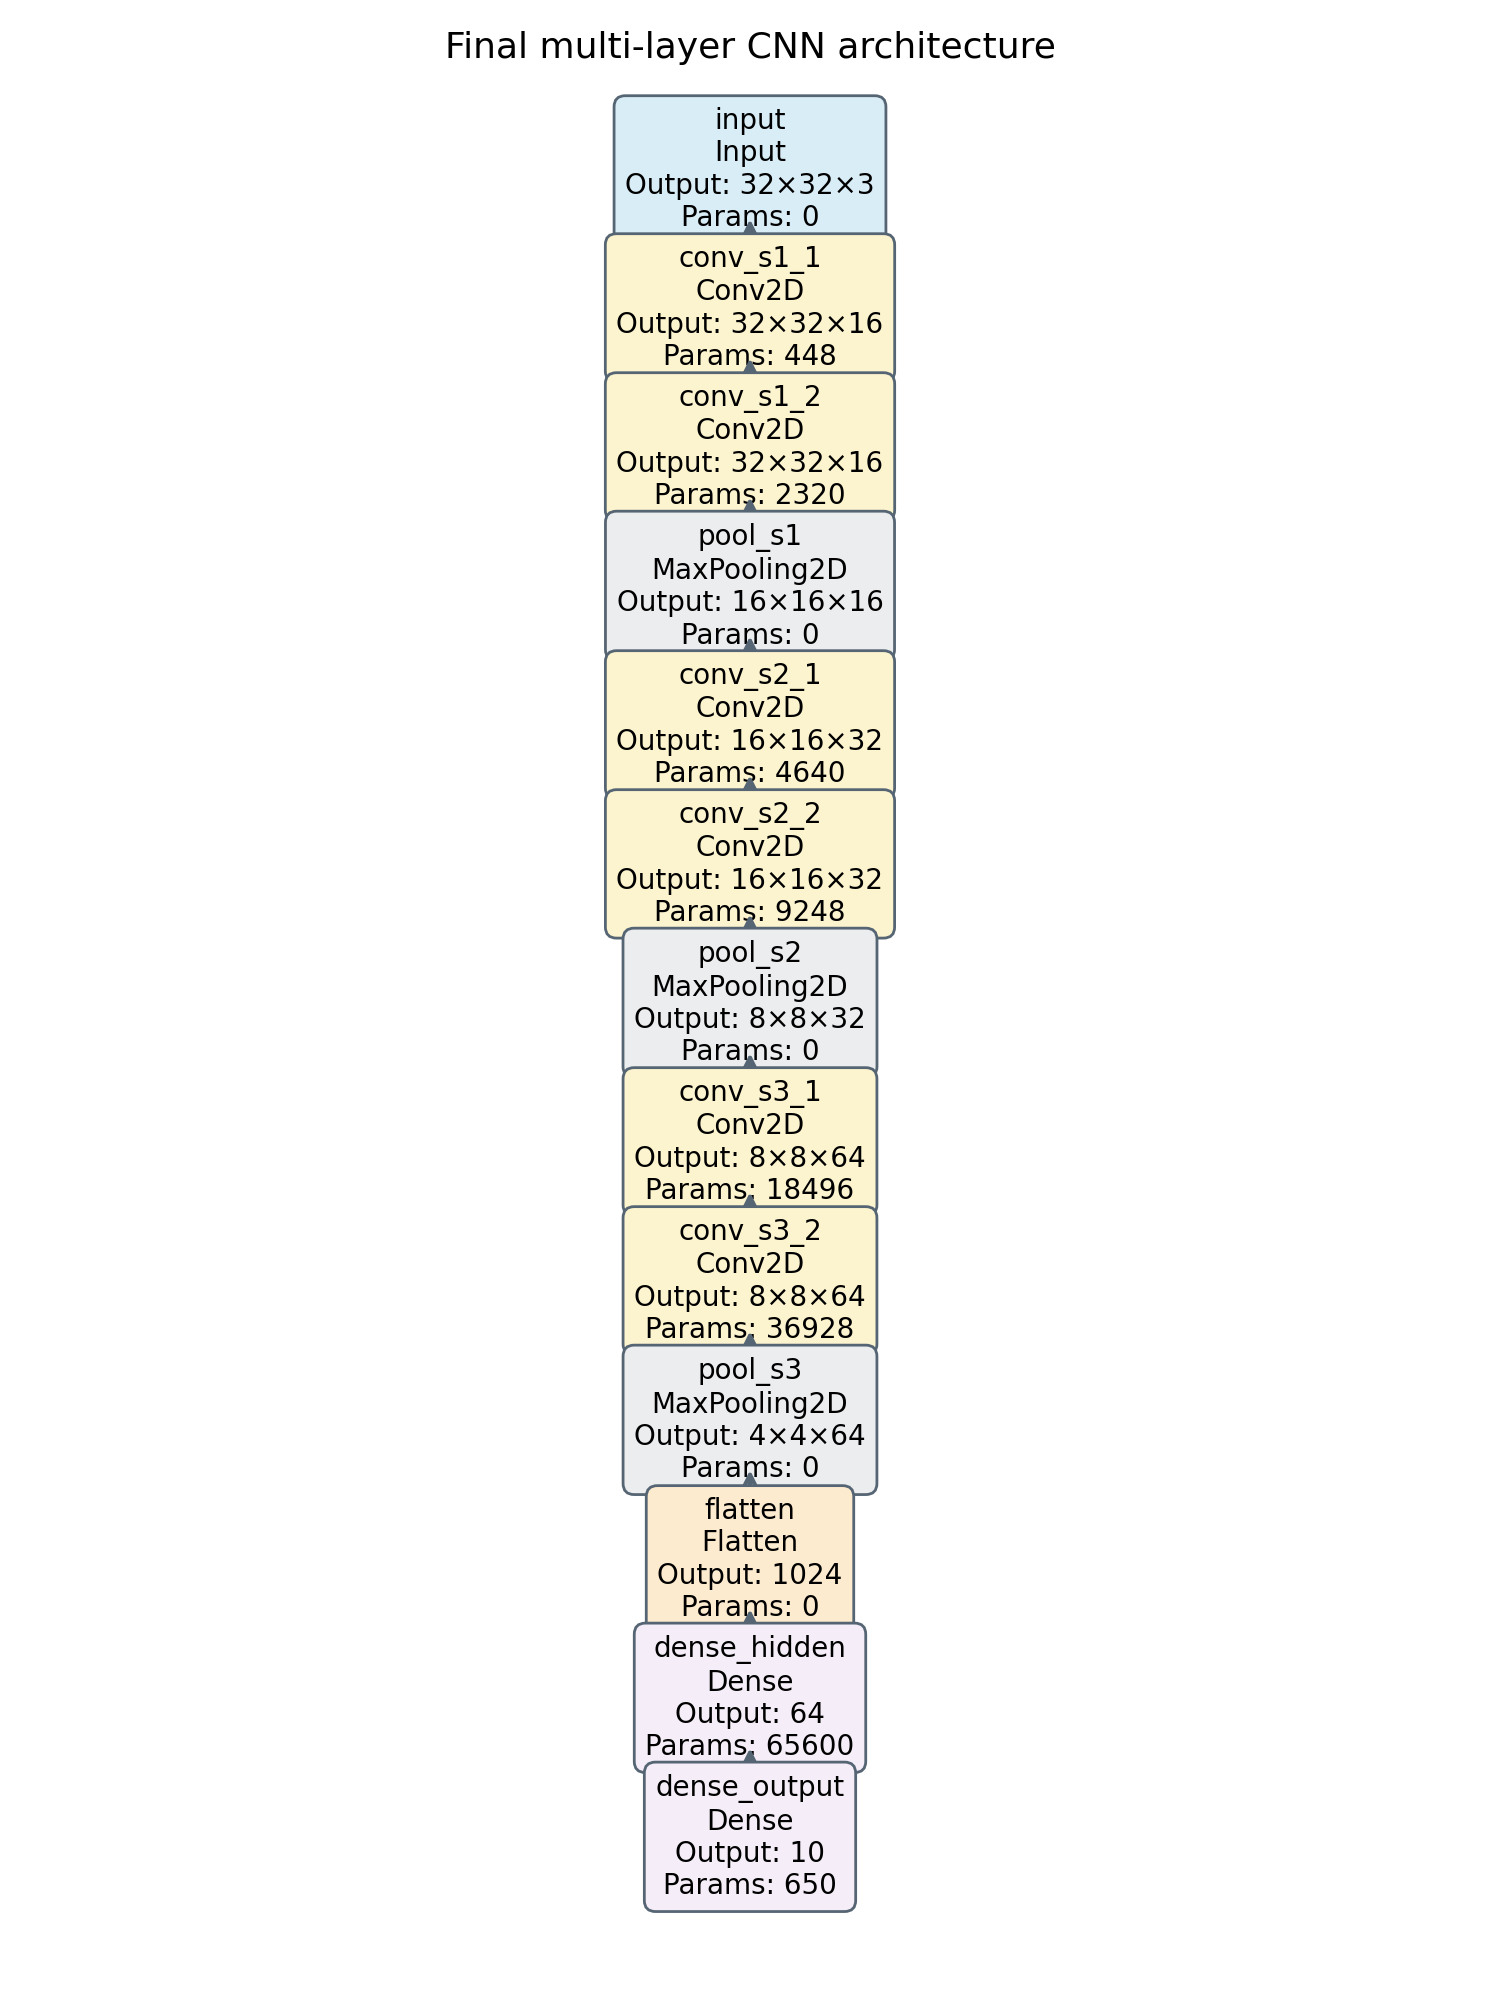
\includegraphics[width=0.8\linewidth]{imgs/section6_final_architecture.png}
\caption{Repr\'esentation graphique du mod\`ele final multi-couches. Le texte interne \`a la figure est laiss\'e en anglais pour garantir un rendu stable.}
\label{fig:section6_architecture}
\end{figure}

\begin{table}[htbp]
\centering
\caption{Hyperparam\`etres retenus pour le mod\`ele final $M3$.}
\label{tab:section6_hyperparameters}
\footnotesize
\begin{tabular}{|l|l|}
\hline
Backbone convolutionnel & $16$-$16$/pool $\rightarrow$ $32$-$32$/pool $\rightarrow$ $64$-$64$/pool \\
Kernel size & $(3,3)$ \\
Padding & \texttt{same} \\
Pool size & $(2,2)$ \\
Dense units & $64$ \\
Dropout apr\`es pooling & $0.25/0.25/0.25$ \\
Dropout avant dense & $0.5$ \\
P\'enalisation $L^2$ & $10^{-4}$ \\
Optimiseur & Adam \\
Learning rate & $10^{-3}$ \\
$\beta_1,\beta_2,\eta$ & $0.9, 0.999, 10^{-7}$ \\
Batch size & $32$ \\
Epochs & $12$ \\
\hline
\end{tabular}
\end{table}

Les courbes d\'apprentissage de la figure~\ref{fig:section6_curves} correspondent \`a un run repr\'esentatif du mod\`ele final avec la graine $42$. Elles montrent une progression r\'eguli\`ere de l'accuracy de validation jusqu\`a l'epoch $11$, o\`u celle-ci atteint $50.5\%$, avant un l\'eger recul \`a $49.2\%$ \`a l'epoch $12$. La \textit{val. loss} suit la m\^eme dynamique, avec un minimum \`a $1.4737$ \`a l'epoch $11$, puis une remont\'ee \`a $1.5332$ \`a l'epoch final. Cette inflexion signale un d\'ebut de sur-apprentissage, mais n'annule pas l'am\'elioration globale observ\'ee par rapport \`a la baseline.

\begin{figure}[htbp]
\centering
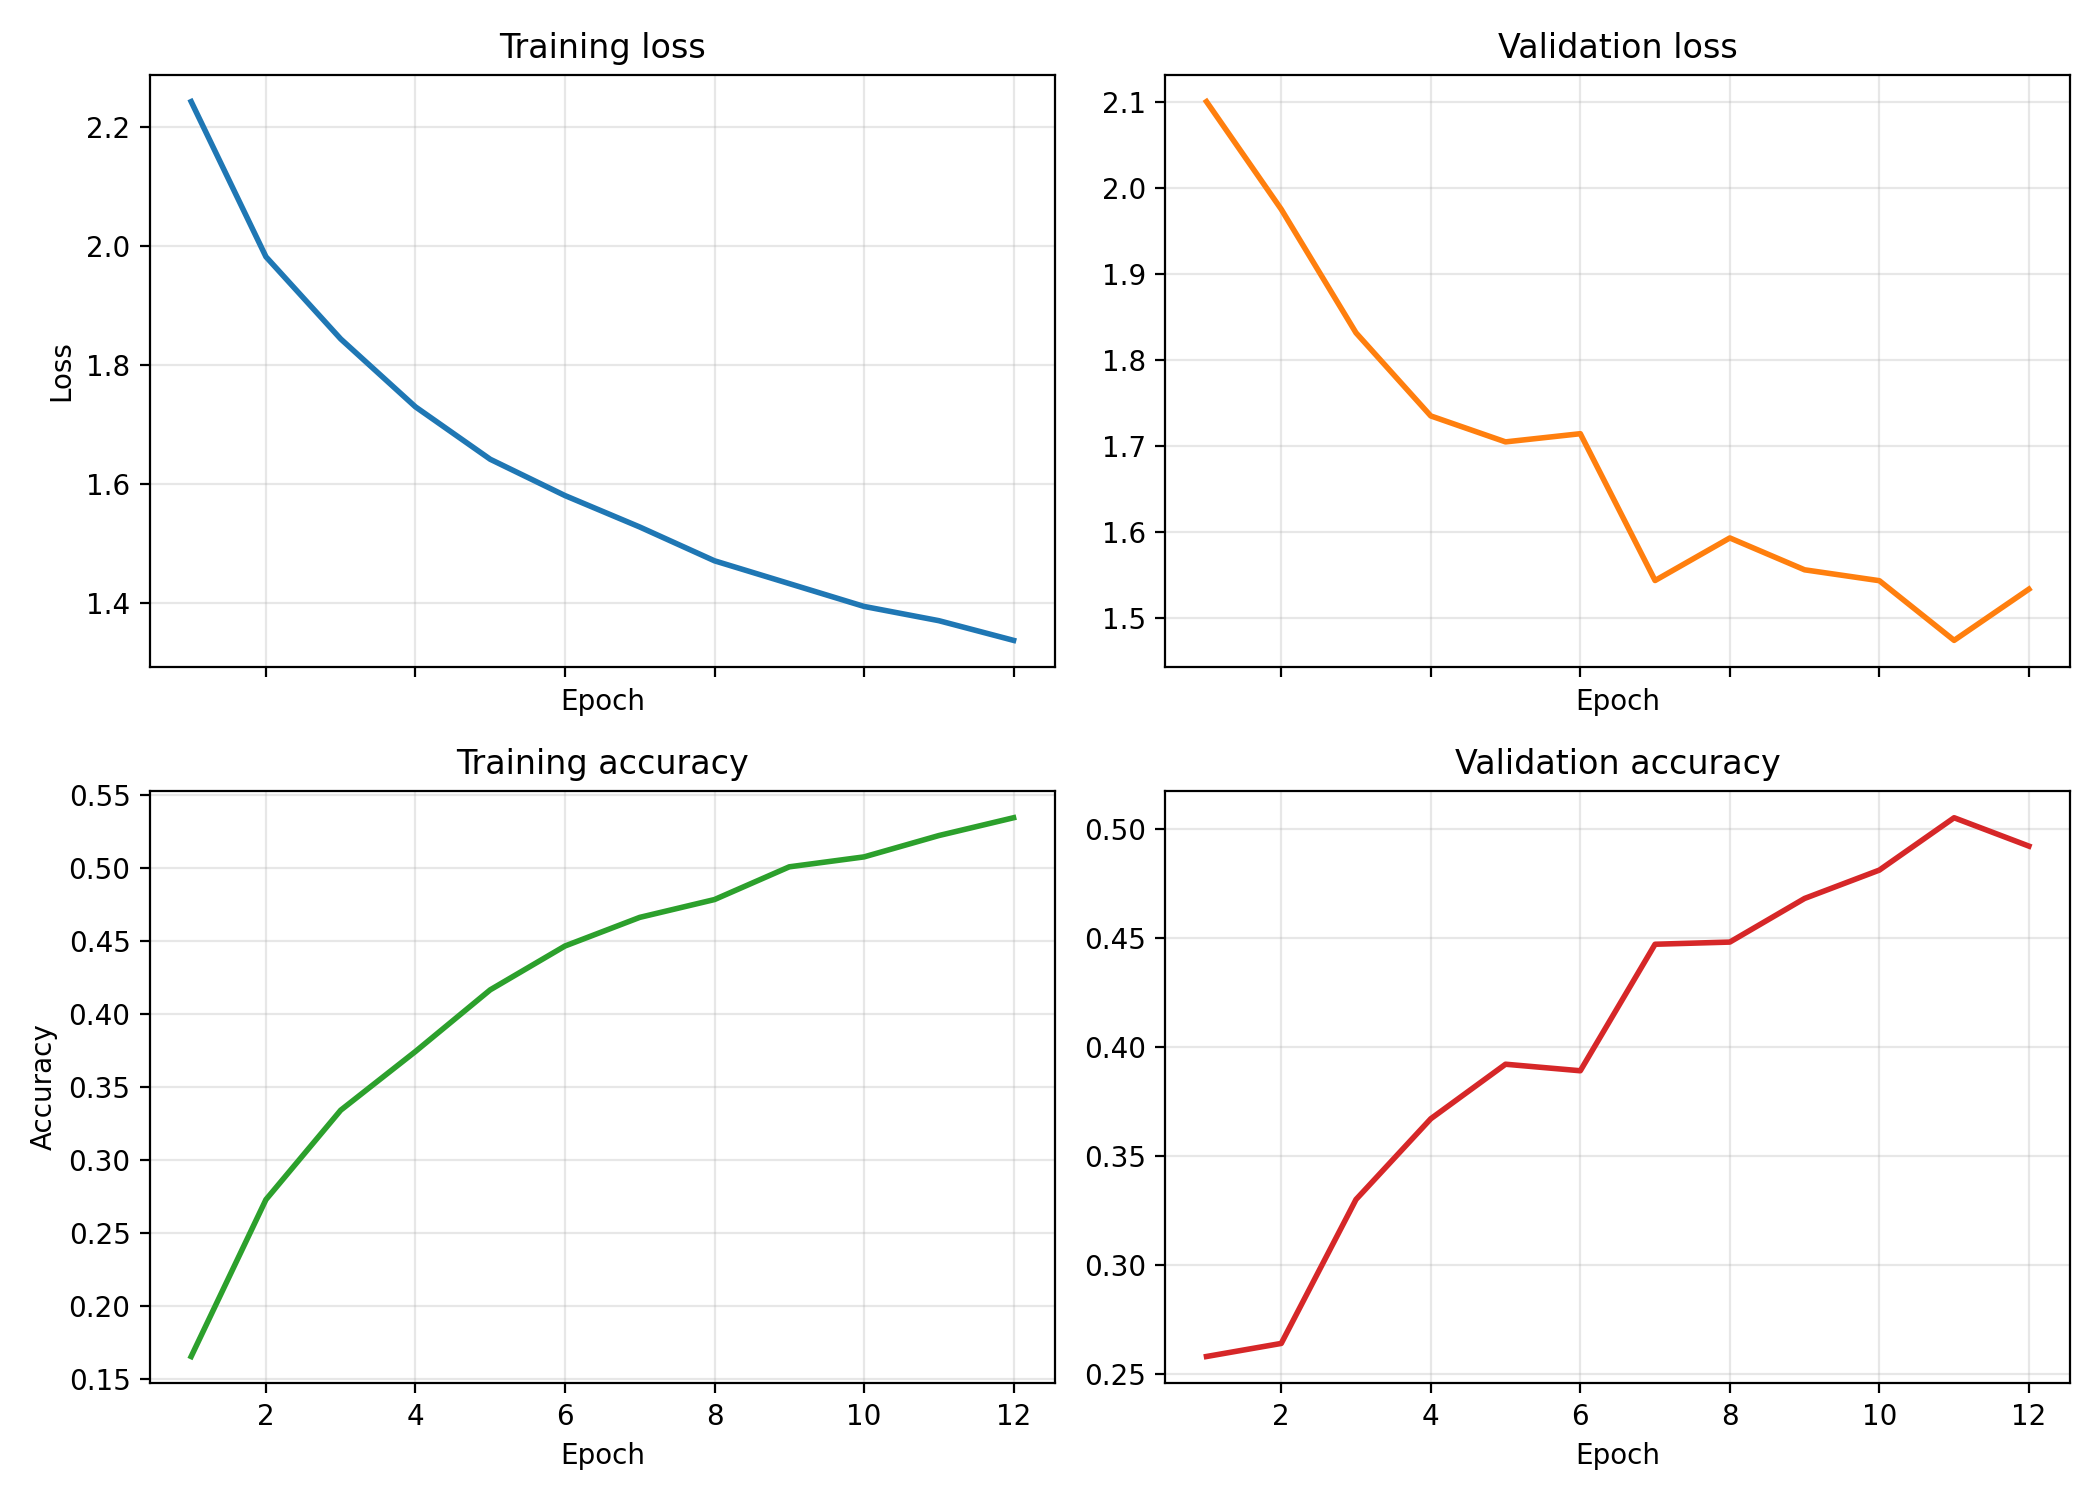
\includegraphics[width=\linewidth]{imgs/section6_final_curves.png}
\caption{Courbes d\'apprentissage du mod\`ele final $M3$ pour le run repr\'esentatif de graine $42$.}
\label{fig:section6_curves}
\end{figure}

Le mod\`ele final atteint sur l'ensemble de test r\'eduit une accuracy de $50.90\%$ et une loss de $1.5058$. Les matrices de confusion de la figure~\ref{fig:section6_confusion} montrent que les classes \textit{frog} ($83.81\%$), \textit{automobile} ($79.80\%$) et \textit{truck} ($72.13\%$) sont les mieux reconnues, tandis que \textit{cat} ($9.68\%$), \textit{bird} ($23.91\%$) et \textit{ship} ($28.92\%$) restent fragiles. Les plus fortes confusions hors diagonale concernent notamment \textit{cat} $\rightarrow$ \textit{dog}, \textit{deer} $\rightarrow$ \textit{frog}, ainsi que \textit{ship} $\rightarrow$ \textit{airplane} ou \textit{automobile}. L'approfondissement am\'eliore donc la s\'eparation de plusieurs classes, mais il ne supprime pas les ambigu\"it\'es visuelles les plus marqu\'ees.

\begin{figure}[htbp]
\centering
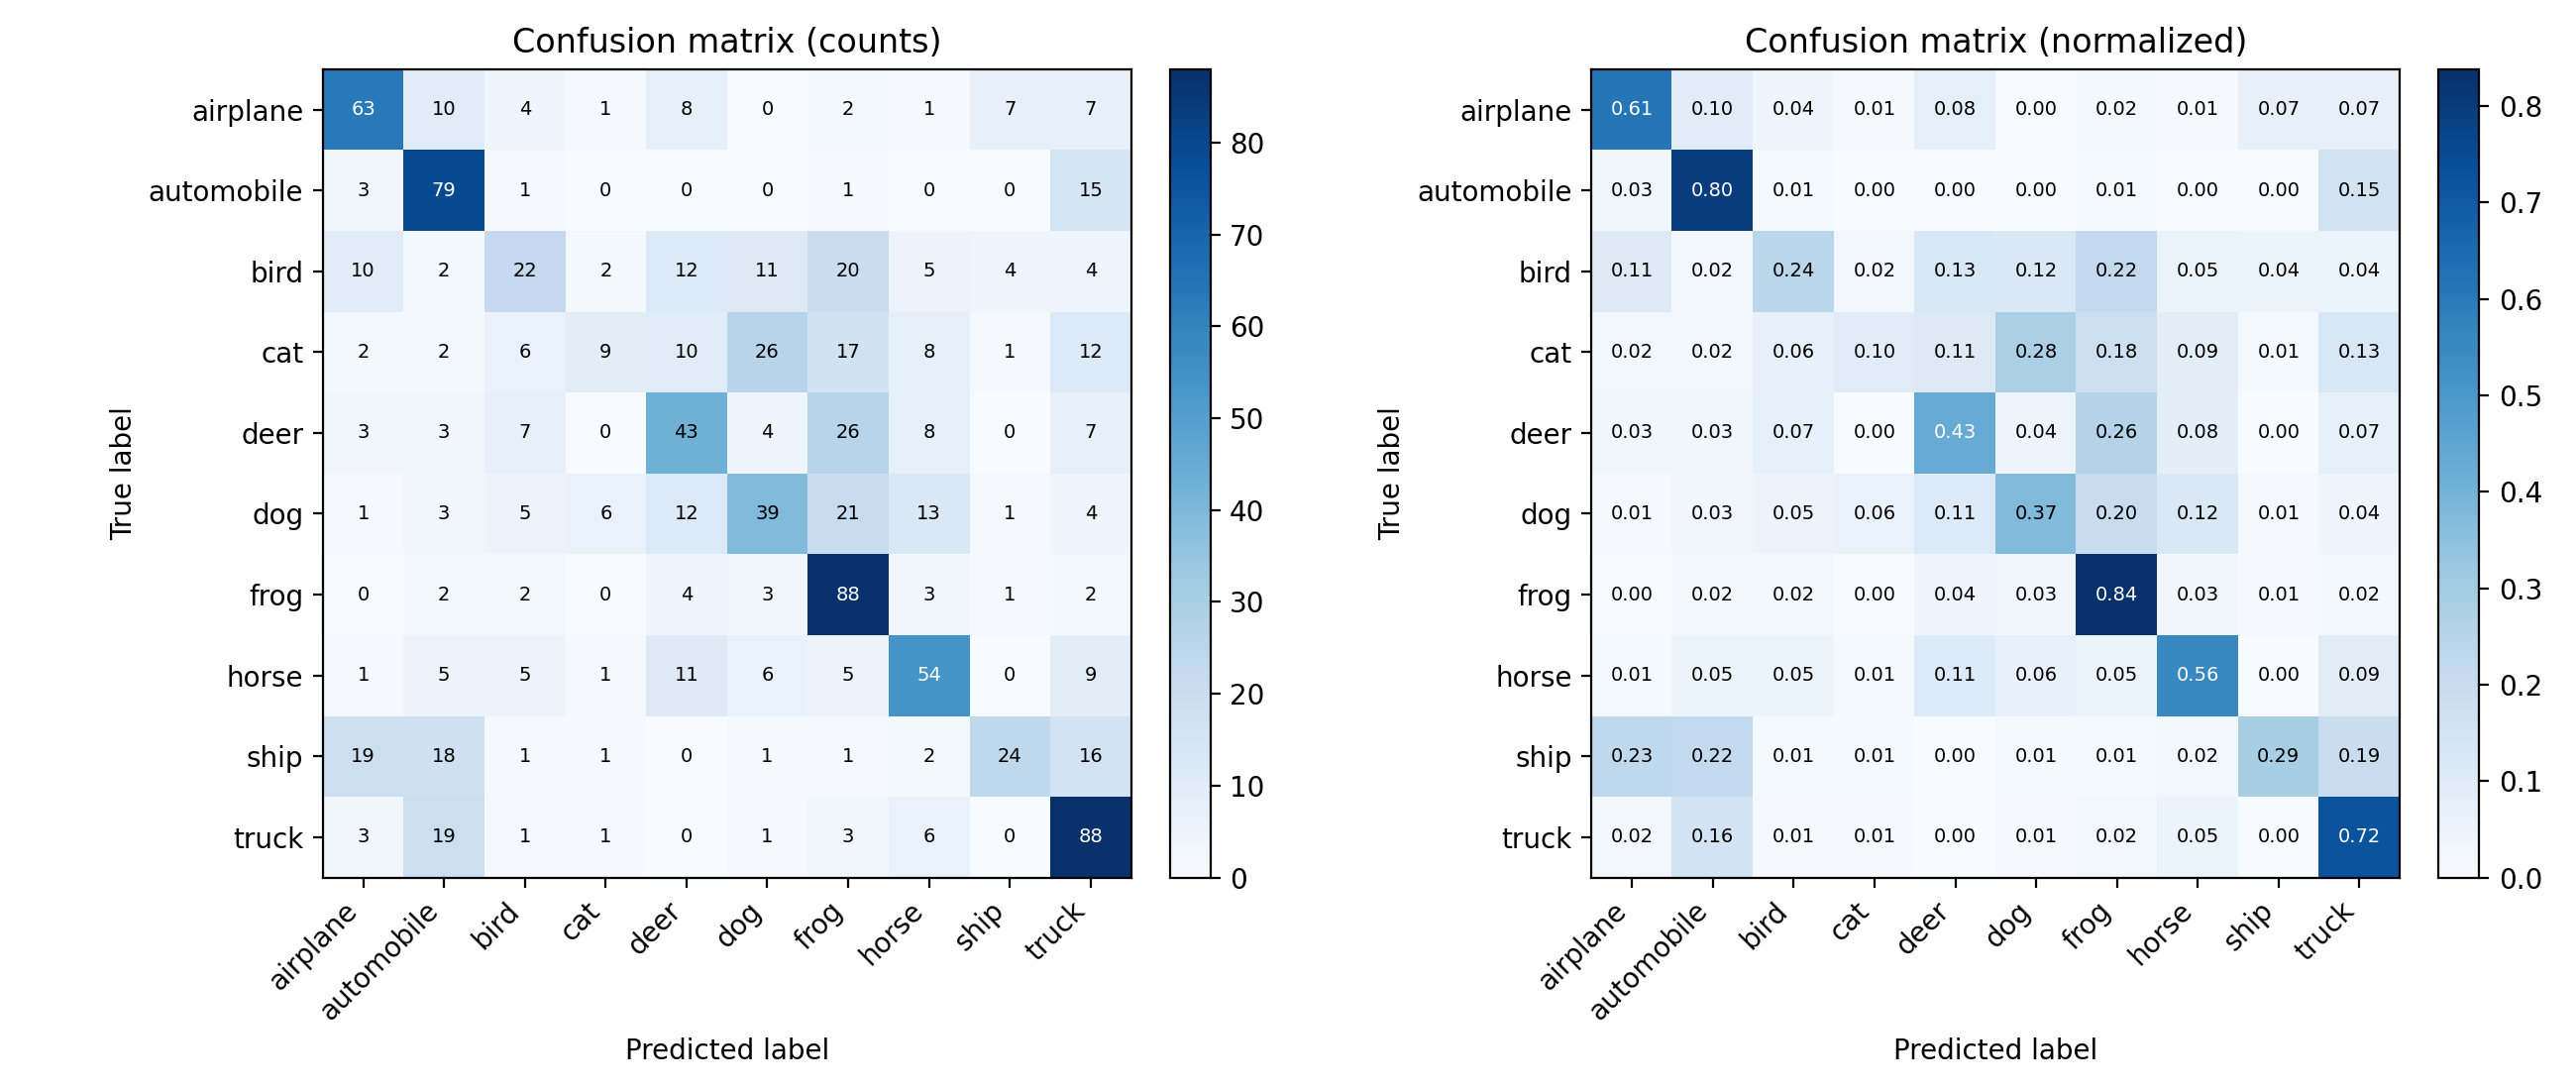
\includegraphics[width=\linewidth]{imgs/section6_final_confusion_matrices.png}
\caption{Matrices de confusion du mod\`ele final : version en effectifs et version normalis\'ee.}
\label{fig:section6_confusion}
\end{figure}

\subsection{Discussion critique : avantages et limites}
L'approfondissement du r\'eseau apporte un gain mesurable et coh\'erent avec le cadre th\'eorique du cours. En empilant plusieurs couches convolutionnelles, le mod\`ele retient des caract\'eristiques plus hi\'erarchiques et voit son champ r\'ecepteur effectif s'agrandir au fil des couches. Cette structuration se traduit ici par une am\'elioration de l'accuracy de validation de $42.30\%$ \`a $50.80\%$ entre $M0$ et $M3$, sans explosion du nombre total de param\`etres. Le gain ne provient donc pas d'une seule augmentation massive de la taille du classifieur dense, mais bien d'une meilleure exploitation de la partie convolutionnelle.

La comparaison entre $M2$ et $M3$ montre en outre que la profondeur seule ne suffit pas. \`A backbone identique, la r\'egularisation explicite de $M3$ am\'eliore nettement la validation et abaisse la \textit{val. loss}. Le \textit{dropout} et la p\'enalisation $L^2$ jouent donc ici le r\^ole attendu : ils limitent la co-adaptation des neurones et contraignent la norme des poids, ce qui devient utile sur un sous-ensemble d'apprentissage aussi restreint.

Les limites du mod\`ele restent n\'eanmoins visibles. D'abord, le co\^ut calculatoire augmente sensiblement : $M3$ exige pr\`es de trois fois plus de temps par epoch que la baseline. Ensuite, la performance absolue demeure mod\'er\'ee sur le test r\'eduit, avec $50.90\%$ d\'accuracy, ce qui montre que la profondeur ne compense ni la petite taille du corpus d\'entra\^inement, ni les ambigu\"it\'es visuelles fortes entre certaines classes. Enfin, les courbes du run repr\'esentatif montrent un d\'ebut de sur-apprentissage en fin d\'entra\^inement, ce qui sugg\`ere que le budget de $12$ epochs reste proche de la limite utile pour cette architecture et ce protocole.

Sous le protocole retenu, l'ajout de profondeur appara\^it donc justifi\'e lorsque la priorit\'e est la pr\'ecision de validation. Le gain de $8.5$ points par rapport \`a la baseline est substantiel, et il s'accompagne d'un meilleur minimum de \textit{val. loss} ainsi que d'une meilleure s\'eparation de plusieurs classes. En revanche, ce raffinement n'a rien d'universel : son int\'er\^et resterait \`a reconsid\'erer si la contrainte principale devenait le temps de calcul plut\^ot que la performance finale.
